\documentclass[border=3mm, tikz]{standalone}

\usepackage{tikz}
\usepackage{tkz-graph}

% https://chrisphan.com/2017/02/22/adventures-in-tikz-tkz-graph/
% https://tex.stackexchange.com/questions/702253/both-internal-and-external-vertex-labels-in-the-package-tkz-graph

\begin{document}

% Figure 1
\input{fig/cip}
% Figure 2
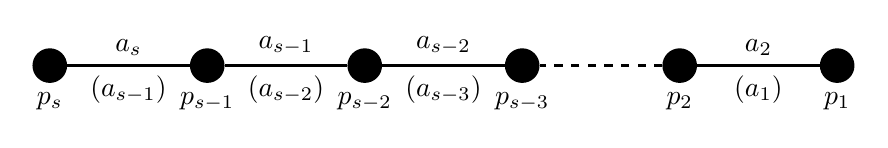
\begin{tikzpicture}

\GraphInit[vstyle=Classic]

\Vertex[Lpos=-90,x=10, y=0, L=$p_{1}$]{p1};
\Vertex[Lpos=-90,x=8, y=0, L=$p_{2}$]{p2};
\Vertex[Lpos=-90,x=6, y=0, L=$p_{s - 3}$]{psm3};
\Vertex[Lpos=-90,x=4, y=0, L=$p_{s - 2}$]{psm2};
\Vertex[Lpos=-90,x=2, y=0, L=$p_{s - 1}$]{psm1};
\Vertex[Lpos=-90,x=0, y=0, L=$p_{s}$]{ps};

\Edge[style ={-},label={$a_{2}$},labelstyle={above}]({p1})({p2})
\Edge[style ={draw=none},label={$(a_{1})$},labelstyle={below}]({p1})({p2})
\Edge[style ={-, dashed}]({p2})({psm3})
\Edge[style ={-},label={$a_{s - 2}$},labelstyle={above}]({psm3})({psm2})
\Edge[style ={draw=none},label={$(a_{s - 3})$},labelstyle={below}]({psm3})({psm2})
\Edge[style ={-},label={$a_{s - 1}$},labelstyle={above}]({psm2})({psm1})
\Edge[style ={draw=none},label={$(a_{s - 2})$},labelstyle={below}]({psm2})({psm1})
\Edge[style ={-},label={$a_{s}$},labelstyle={above}]({psm1})({ps})
\Edge[style ={draw=none},label={$(a_{s - 1})$},labelstyle={below}]({psm1})({ps})

\end{tikzpicture}

% Figure 3
\GraphInit[vstyle=Classic]

\Vertex[Lpos=-90, x=0, y=0, L=$v$]{v};
\Vertex[Lpos=-90, x=2, y=0, L=$p_{1}$]{p1};

\Edge[style ={-},label={$a_{1}$},labelstyle={above}]({v})({p1})
\Edge[style ={draw=none},label={$(a_{2})$},labelstyle={below}]({v})({p1})

% Figure 4
\GraphInit[vstyle=Classic]

\Vertex[Lpos=-90, x=0, y=0, L=$v$]{v};
\Vertex[Lpos=-90, x=2, y=0, L=$p_{1}$]{p1};
\Vertex[Lpos=-90, x=4, y=0, L=$p_{2}$]{p2};

\Edge[style ={-},label={$a_{1}$},labelstyle={above}]({v})({p1})
\Edge[style ={draw=none},label={$(a_{2})$},labelstyle={below}]({v})({p1})
\Edge[style ={-},label={$a_{2}$},labelstyle={above}]({p1})({p2})
\Edge[style ={draw=none},label={},labelstyle={below}]({p1})({p2})

% Figure 5
\input{fig/cip-two-edge-flip}
% Figure 6
\input{fig/cip-three-edge}
% Figure 7
\begin{tikzpicture}

\GraphInit[vstyle=Classic]

\Vertex[Lpos=-90, x=0, y=0, L=$p_{1}$]{p1};
\Vertex[Lpos=-90, x=2, y=0, L=$p_{2}$]{p2};
\Vertex[Lpos=-90, x=4, y=0, L=$p_{3}$]{p3};
\Vertex[Lpos=-90, x=6, y=0, L=$p_{t - 1}$]{ptm1};
\Vertex[Lpos=-90, x=8, y=0, L=$p_{t}$]{pt};
\Vertex[Lpos=-90, x=10, y=0, L=$p_{t + 1}$]{ptp1};
\Vertex[Lpos=-90, x=12, y=0, L=$p_{t + 2}$]{ptp2};
\Vertex[Lpos=-90, x=14, y=0, L=$p_{s - 1}$]{psm1};
\Vertex[Lpos=-90, x=16, y=0, L=$p_{s}$]{ps};

\Edge[style ={-},label={$a_{1}$},labelstyle={above}]({p1})({p2})
\Edge[style ={draw=none},label={$(a_{2})$},labelstyle={below}]({p1})({p2})
\Edge[style ={-},label={$a_{2}$},labelstyle={above}]({p2})({p3})
\Edge[style ={draw=none},label={$(a_{3})$},labelstyle={below}]({p2})({p3})
\Edge[style ={-, dashed},labelstyle={above}]({p3})({ptm1})
\Edge[style ={-},label={$a_{t - 1}$},labelstyle={above}]({ptm1})({pt})
\Edge[style ={draw=none},label={$(a_{t})$},labelstyle={below}]({ptm1})({pt})
\Edge[style ={-},label={$a_{t}$},labelstyle={above}]({pt})({ptp1})
\Edge[style ={draw=none},label={$(a_{t + 1})$},labelstyle={below}]({pt})({ptp1})
\Edge[style ={-},label={$a_{t + 1}$},labelstyle={above}]({ptp1})({ptp2})
\Edge[style ={draw=none},label={$(a_{t + 2})$},labelstyle={below}]({ptp1})({ptp2})
\Edge[style ={-, dashed},labelstyle={above}]({ptp2})({psm1})
\Edge[style ={-},label={$a_{s - 1}$},labelstyle={above}]({psm1})({ps})
\Edge[style ={draw=none},label={$(a_{s})$},labelstyle={below}]({psm1})({ps})

% https://tex.stackexchange.com/questions/430072/longer-curly-braces-in-tikz
\draw [thick, decorate,decoration={brace,amplitude=10pt},yshift=2pt] (0, 0.3) -- (7.9, 0.3) node [black,midway,yshift=16pt] {$P_{1}$};
\draw [thick, decorate,decoration={brace,amplitude=10pt},yshift=2pt] (8.1, 0.3) -- (16, 0.3) node [black,midway,yshift=16pt] {$P_{2}$};

\draw [arrows = {-Stealth[length=10pt, inset=2pt]}] (8.5, 1.5) -- (8, 0.5);

\node[text width = 1cm] at (9.2, 1.5) {cut};

\end{tikzpicture}

% Figure 8
\begin{tikzpicture}

\GraphInit[vstyle=Classic]

\Vertex[Lpos=-90, x=0, y=0, L=$p_{1}$]{p1};
\Vertex[Lpos=-90, x=2, y=0, L=$p_{2}$]{p2};
\Vertex[Lpos=-90, x=4, y=0, L=$p_{3}$]{p3};
\Vertex[Lpos=-90, x=6, y=0, L=$p_{t - 1}$]{ptm1};
\Vertex[Lpos=-90, x=8, y=0, L=$p_{t}$]{pt};
\Vertex[Lpos=-90, x=10, y=0, L=$p_{t + 1}$]{ptp1};
\Vertex[Lpos=-90, x=12, y=0, L=$p_{t + 2}$]{ptp2};
\Vertex[empty, x=14, y=0]{p};

\Edge[style ={-},label={$a_{1}$},labelstyle={above}]({p1})({p2})
\Edge[style ={draw=none},label={$(a_{2})$},labelstyle={below}]({p1})({p2})
\Edge[style ={-},label={$a_{2}$},labelstyle={above}]({p2})({p3})
\Edge[style ={draw=none},label={$(a_{3})$},labelstyle={below}]({p2})({p3})
\Edge[style ={-, dashed},labelstyle={above}]({p3})({ptm1})
\Edge[style ={-},label={$a_{t - 1}$},labelstyle={above}]({ptm1})({pt})
\Edge[style ={draw=none},label={$(a_{t})$},labelstyle={below}]({ptm1})({pt})
\Edge[style ={-},label={$a_{t + 1}$},labelstyle={above}]({pt})({ptp1})
\Edge[style ={-},label={$a_{t + 2}$},labelstyle={above}]({ptp1})({ptp2})
\Edge[style ={-, dashed},labelstyle={above}]({ptp2})({p})

\draw [arrows = {-Stealth[length=10pt, inset=2pt]}] (8.5, 1.5) -- (8, 0.5);
\node[text width = 1cm] at (9.2, 1.5) {cut};

\end{tikzpicture}

% Figure 9
\begin{tikzpicture}

\GraphInit[vstyle=Classic]

\Vertex[empty, x=0, y=0]{p};
\Vertex[Lpos=-90, x=2, y=0, L=$p_{t - 2}$]{ptm2};
\Vertex[Lpos=-90, x=4, y=0, L=$p_{t - 1}$]{ptm1};
\Vertex[Lpos=-90, x=6, y=0, L=$p_{t}$]{pt};
\Vertex[Lpos=-90, x=8, y=0, L=$p_{t + 1}$]{ptp1};
\Vertex[Lpos=-90, x=10, y=0, L=$p_{t + 2}$]{ptp2};
\Vertex[Lpos=-90, x=12, y=0, L=$p_{s - 1}$]{psm1};
\Vertex[Lpos=-90, x=14, y=0, L=$p_{s}$]{ps};

\Edge[style ={-, dashed},labelstyle={above}]({p})({ptm2})
\Edge[style ={-},label={$a_{t - 2}$},labelstyle={above}]({ptm2})({ptm1})
\Edge[style ={-},label={$a_{t - 1}$},labelstyle={above}]({ptm1})({pt})
\Edge[style ={-},label={$a_{t}$},labelstyle={above}]({pt})({ptp1})
\Edge[style ={draw=none},label={$(a_{t + 1})$},labelstyle={below}]({pt})({ptp1})
\Edge[style ={-},label={$a_{t + 1}$},labelstyle={above}]({ptp1})({ptp2})
\Edge[style ={draw=none},label={$(a_{t + 2})$},labelstyle={below}]({ptp1})({ptp2})
\Edge[style ={-, dashed},labelstyle={above}]({ptp2})({psm1})
\Edge[style ={-},label={$a_{s - 1}$},labelstyle={above}]({psm1})({ps})
\Edge[style ={draw=none},label={$(a_{s})$},labelstyle={below}]({psm1})({ps})

\draw [arrows = {-Stealth[length=10pt, inset=2pt]}] (6.5, 1.5) -- (6, 0.5);
\node[text width = 1cm] at (7.2, 1.5) {cut};

\end{tikzpicture}

% Figure 10
\GraphInit[vstyle=Classic]

\Vertex[Lpos=-90, x=0, y=0, L=$p_{1}$]{p1};
\Vertex[Lpos=-90, x=2, y=0, L=$p_{2}$]{p2};
\Vertex[Lpos=-90, x=4, y=0, L=$p_{3}$]{p3};
\Vertex[Lpos=-90, x=6, y=0, L=$p_{4}$]{p4};
\Vertex[Lpos=-90, x=8, y=0, L=$p_{t}$]{pt};
\Vertex[Lpos=-90, x=10, y=0, L=$p_{t + 1}$]{ptp1};
\Vertex[Lpos=-90, x=12, y=0, L=$p_{t + 2}$]{ptp2};
% https://tex.stackexchange.com/questions/265780/invisible-vertices-with-tkz-graph
\Vertex[empty,x=14, y=0]{p};

\Edge[style ={-},label={$a_{1}$},labelstyle={above}]({p1})({p2})
\Edge[style ={draw=none},label={$(a_{2})$},labelstyle={below}]({p1})({p2})
\Edge[style ={-},label={$a_{2}$},labelstyle={above}]({p2})({p3})
\Edge[style ={draw=none},label={$(a_{1})$},labelstyle={below}]({p2})({p3})
\Edge[style ={-},label={$a_{1}$},labelstyle={above}]({p3})({p4})
\Edge[style ={draw=none},label={$(a_{2})$},labelstyle={below}]({p3})({p4})
\Edge[style ={-},label={$a_{2}$},labelstyle={above}]({p4})({pt})
\Edge[style ={draw=none},label={$(a_{1})$},labelstyle={below}]({p4})({pt})
\Edge[style ={-},label={$a_{3}$},labelstyle={above}]({pt})({ptp1})
\Edge[style ={-},label={$a_{4}$},labelstyle={above}]({ptp1})({ptp2})
\Edge[style ={-},label={},labelstyle={above}]({ptp2})({p})

% Figure 11
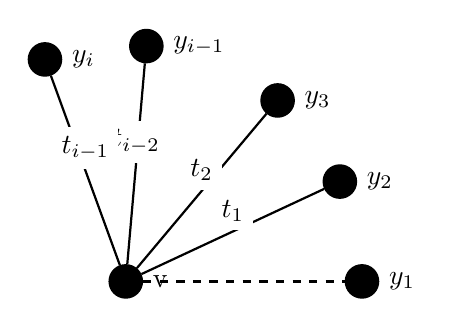
\begin{tikzpicture}
  \GraphInit[vstyle=Classic]

  \Vertex{v}
  \Vertex[a=0, d=3cm, L=$y_{1}$]{y1}
  \Vertex[a=25, d=3cm, L=$y_{2}$]{y2}
  \Vertex[a=50, d=3cm, L=$y_{3}$]{y3}
  \Vertex[a=85, d=3cm, L=$y_{i-1}$]{yim1}
  \Vertex[a=110, d=3cm, L=$y_{i}$]{yi}

  \Edge[style ={-, dashed}]({v})({y1})
  \Edge[style ={-}, label={$t_{1}$},labelstyle={above}]({v})({y2})
  \Edge[style ={-}, label={$t_{2}$},labelstyle={above}]({v})({y3})
  \Edge[style ={-}, label={$t_{i - 2}$},labelstyle={above}]({v})({yim1})
  \Edge[style ={-}, label={$t_{i - 1}$},labelstyle={above}]({v})({yi})
 
\end{tikzpicture}




\end{document}
